\noindent

\includegraphics[height=1.25cm]{images/pictograms/under_construction}

\includegraphics[height=1.25cm]{images/pictograms/bsc}

\includegraphics[height=1.25cm]{images/pictograms/tools}

\includegraphics[height=1.25cm]{images/pictograms/paraview}

%%%%%%%%%%%%%%%%%%%%%%%%%%%%%%%%%%%%%%%%%%%%%%%%%%%%%%%%%%%%%%%%%%%%%%%%%%%%%%%%%%%%%%%%%%%%%%%%%%%

\begin{flushright} {\tiny {\color{gray} python\_codes/fieldstone\_159/text.tex}} \end{flushright}

%\lstinputlisting[language=bash,basicstyle=\small]{python_codes/template_keywords.key}

\par\noindent\rule{\textwidth}{0.4pt}

\begin{center}
\inpython
{\small Code: \url{https://github.com/cedrict/fieldstone/tree/master/python_codes/fieldstone_159}}
\end{center}

\par\noindent\rule{\textwidth}{0.4pt}

%%%%%%%%%%%%%%%%%%%%%%%%%%%%%%%%%%%%%%%%%%%%%%%%%%%%%%%%%%%%%%%%%%%%%%%%%%%%%%%%%%%%%%%%%%%%%%%%%%%

The goal of this \stone is to explore, check and plot the yield envelopes of 
the main plastic yield criteria.
We will here focus on:
\begin{itemize} 
\item von Mises
\item Tresca
\item Mohr-Coulomb
\item Drucker-Prager (all three variants)
\end{itemize} 
The four models are parameterized by a cohesion $c$ and an angle of friction $\phi$. 

The code works as follows: We will explore a stress space $[-\sigma_{max},\sigma_{max}]^3$.
For each point inside this domain, we compute the 1st, 2nd and 3rd moment invariants, i.e.
\[
\III_1(), \qquad \III_2(), \qquad \III_3(), \qquad \uptheta_{\rm L}
\] 
At each point we will then evaluate the yield function $\FFF$. 
If {\python make\_vtu} is True, a (very large) vtu file will be produced (in this 
case nnx should not exceed 200).
The code exports the point that fulfill $\FFF=0$ within 20kPa. 
which allows to trace the yield envelopes.
The same can be achieved by opening the vtu file and looking at zero isocontours of each $\FFF$ field.

We set $c=20MPa$ and $\phi=20\degree$. After trial an error, we set $\sigma_{max}=60MPa$.

\begin{center}
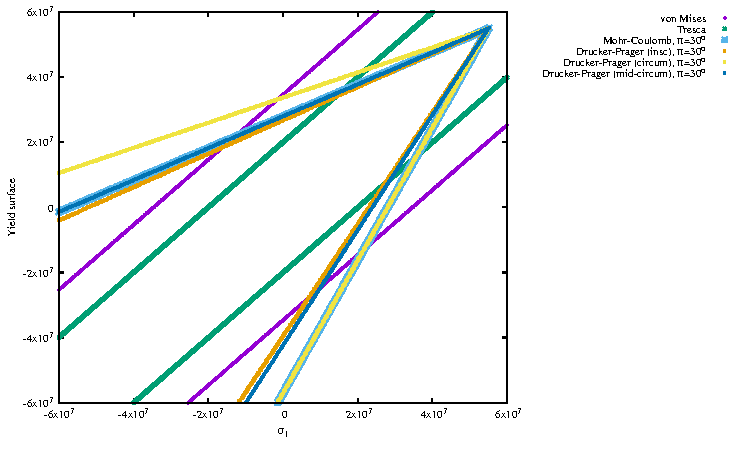
\includegraphics[width=12cm]{python_codes/fieldstone_159/images/surfaces_xy.pdf}
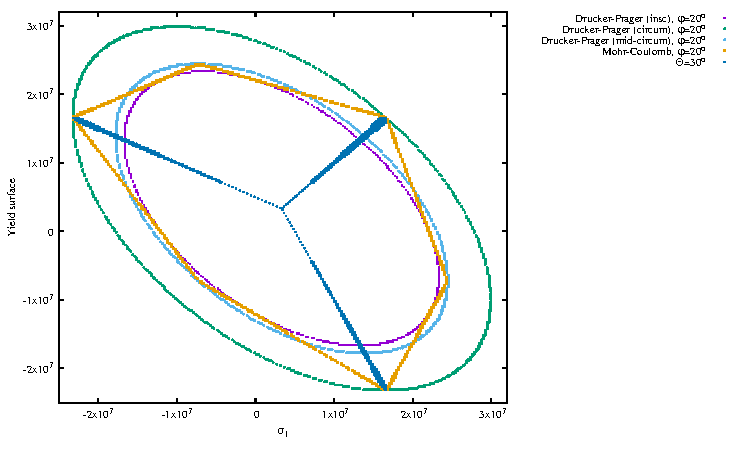
\includegraphics[width=12cm]{python_codes/fieldstone_159/images/surfaces_plane.pdf}
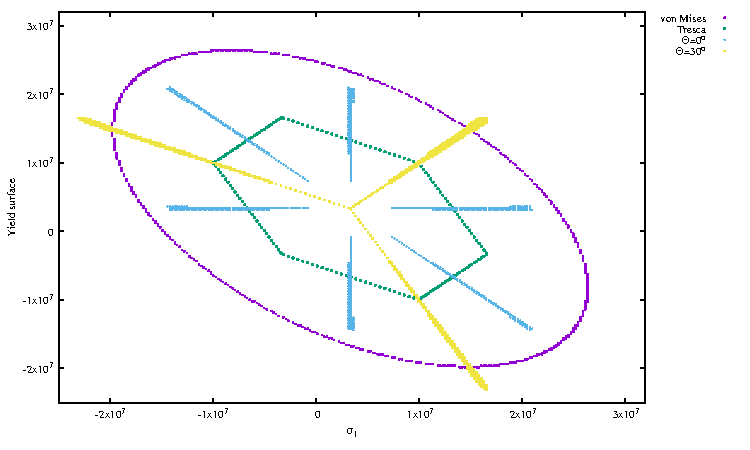
\includegraphics[width=12cm]{python_codes/fieldstone_159/images/surfaces_plane2.pdf}\\
{\captionfont Obtained with nnx=512}.
\end{center}

I need to fix pi3 file ?!




